% Final report. Compile with: pdflatex main && bibtex main && pdflatex main && pdflatex main
% Tables, figures and the numbers quoted in the text are generated by
%   python scripts/06_make_report.py
% from the files under results/. Nothing in generated/ is typed by hand.
\documentclass[11pt]{article}
\usepackage[final]{acl}
\usepackage{times}
\usepackage{latexsym}
\usepackage[T1]{fontenc}
\usepackage[utf8]{inputenc}
\usepackage{microtype}
\usepackage{graphicx}
\usepackage{booktabs}
\usepackage{amsmath}
\usepackage{xcolor}
\usepackage{enumitem}
\usepackage{tikz}
\usetikzlibrary{positioning,arrows.meta,calc}
\setlist{nosep,leftmargin=*}

% ---- generated content --------------------------------------------------------------
\newcommand{\pending}{\textcolor{red}{[run]}}
\IfFileExists{generated/numbers.tex}{\providecommand{\GeneratorModel}{llama3.1:8b}
\providecommand{\JudgeModel}{qwen2.5:7b}
\providecommand{\TrecDocs}{171,332}
\providecommand{\TrecPassages}{238,432}
\providecommand{\TrecDev}{15}
\providecommand{\TrecTest}{35}
\providecommand{\BmKone}{1.6}
\providecommand{\BmB}{0.50}
\providecommand{\DenseModel}{MiniLM-L6}
\providecommand{\NdcgBm}{0.620}
\providecommand{\NdcgDense}{0.576}
\providecommand{\NdcgHybrid}{0.698}
\providecommand{\PubDocs}{950}
\providecommand{\PubAnswerable}{100}
\providecommand{\PubOut}{30}
\providecommand{\TopK}{3}
\providecommand{\RagWins}{40}
\providecommand{\CbWins}{8}
\providecommand{\JudgeTies}{52}
\providecommand{\AbstainAcc}{100.0}
\providecommand{\OverRefusal}{9.0}
\providecommand{\RrfTestCaught}{63.3}
\providecommand{\RrfTestRefused}{13.0}
\providecommand{\RrfTestAuroc}{0.776}
\providecommand{\CeTestCaught}{96.7}
\providecommand{\CeTestRefused}{8.0}
\providecommand{\CeTestAuroc}{0.986}
\providecommand{\CitePrec}{51.2}
\providecommand{\CiteRec}{36.3}
\providecommand{\Faithfulness}{90.9}
\providecommand{\NliPairs}{165}
\providecommand{\NliWindow}{2}
\providecommand{\NliJudgeRate}{84.2}
\providecommand{\NliWholeRate}{21.2}
\providecommand{\NliWholeKappa}{0.10}
\providecommand{\NliWindowRate}{56.4}
\providecommand{\NliWindowKappa}{0.28}
}{}
% fall-backs so the paper compiles before the experiments have been run
\providecommand{\GeneratorModel}{\pending}\providecommand{\JudgeModel}{\pending}
\providecommand{\TrecDocs}{171K}\providecommand{\TrecPassages}{\pending}
\providecommand{\TrecDev}{15}\providecommand{\TrecTest}{35}
\providecommand{\BmKone}{\pending}\providecommand{\BmB}{\pending}\providecommand{\DenseModel}{MiniLM-L6}
\providecommand{\NdcgBm}{\pending}\providecommand{\NdcgDense}{\pending}\providecommand{\NdcgHybrid}{\pending}
\providecommand{\PubDocs}{950}\providecommand{\PubAnswerable}{100}\providecommand{\PubOut}{30}\providecommand{\TopK}{\pending}
\providecommand{\RagWins}{\pending}\providecommand{\CbWins}{\pending}\providecommand{\JudgeTies}{\pending}
\providecommand{\AbstainAcc}{\pending}\providecommand{\OverRefusal}{\pending}
\providecommand{\RrfTestAuroc}{\pending}\providecommand{\RrfTestCaught}{\pending}\providecommand{\RrfTestRefused}{\pending}
\providecommand{\CeTestAuroc}{\pending}\providecommand{\CeTestCaught}{\pending}\providecommand{\CeTestRefused}{\pending}
\providecommand{\CitePrec}{\pending}\providecommand{\CiteRec}{\pending}\providecommand{\Faithfulness}{\pending}
\providecommand{\NliPairs}{\pending}\providecommand{\NliWindow}{2}\providecommand{\NliJudgeRate}{\pending}
\providecommand{\NliWholeRate}{\pending}\providecommand{\NliWholeKappa}{\pending}
\providecommand{\NliWindowRate}{\pending}\providecommand{\NliWindowKappa}{\pending}
\providecommand{\HandcheckResult}{50 hand-checked comparisons \pending{} (the team fills in
  \texttt{judge\_handcheck.csv}, then runs \texttt{score\_handcheck.py} and \texttt{06\_make\_report.py})}

\newcommand{\gen}[1]{\IfFileExists{generated/#1.tex}{\input{generated/#1.tex}}{%
  \begin{center}\fbox{\parbox{0.92\linewidth}{\small\itshape Table \texttt{\detokenize{#1}} is generated
  when the experiments are run (\texttt{./run\_all.sh}).}}\end{center}}}
\newcommand{\genfig}[3]{\IfFileExists{figures/#1.pdf}{%
  \begin{figure}[t]\centering\includegraphics[width=#2]{figures/#1.pdf}\caption{#3}\label{fig:#1}\end{figure}}{}}
\newcommand{\genfigwide}[3]{\IfFileExists{figures/#1.pdf}{%
  \begin{figure*}[t]\centering\includegraphics[width=#2]{figures/#1.pdf}\caption{#3}\label{fig:#1}\end{figure*}}{}}

\title{A Private, Citation-Grounded RAG Search Engine\\over Local Document Collections}

\author{Sai Nithin Maddi \\ NetID: sai\_nithin \And Sumanth Reddy \\ NetID: madsum01 \And Zhiyan Song \\ NetID: jane\_song}

\begin{document}
\maketitle

\begin{abstract}
Organisations that hold sensitive documents cannot paste them into a hosted chatbot, and a
fluent but unsupported answer is worse for them than no answer. We built a search engine that
keeps everything on one machine: it indexes a private collection, retrieves passages with a
hybrid of BM25 and dense embeddings, and has a locally hosted 7--8B LLM answer only from those
passages, with inline citations, or decline with ``not found in the knowledge base''.
We evaluate each stage on public stand-ins for private data. On TREC-COVID
(\TrecTest{} held-out topics) BM25, dense and hybrid retrieval reach nDCG@10 of \NdcgBm,
\NdcgDense{} and \NdcgHybrid. On \PubAnswerable{} PubMedQA questions an LLM judge prefers the
grounded answer over the same model answering closed-book in \RagWins{} cases and the
closed-book answer in \CbWins. The system declines \AbstainAcc\% of \PubOut{} questions whose
source is not in the collection while wrongly declining \OverRefusal\% of answerable ones;
ALCE-style citation precision is \CitePrec\% and RAGAs-style faithfulness \Faithfulness\%.
We ablate chunk size, top-$k$, fusion method and re-ranking, add a lightweight entity-graph
extension, and categorise the failures. Code, data splits and every table are reproducible
with one command.
\end{abstract}

\section{Introduction}

Hospitals, law firms and companies hold documents they are not allowed to send to a third
party and do not want used to train a model. Fine-tuning a model on such data is expensive,
bakes the data into weights where it is hard to update or delete, and still hallucinates.
Retrieval-augmented generation \citep{lewis2020rag} keeps the knowledge in an index that can
be updated by re-indexing a file, and lets every claim be traced to a source.

Document chat already exists in commercial copilots and in open-source tools such as
PrivateGPT, GPT4All LocalDocs and AnythingLLM, and in frameworks such as LangChain,
LlamaIndex and Haystack. We do not claim the idea is new. Our prototype differs in three
ways that matter in sensitive settings:

\begin{itemize}
\item \textbf{A fully local pipeline.} Indexing, retrieval, re-ranking, generation and
evaluation all run on a laptop. No document, query or retrieved snippet leaves the machine;
the LLM client refuses a non-local host unless that is explicitly allowed.
\item \textbf{A measured comparison of retrieval strategies inside the same application.}
BM25, dense retrieval, their fusion and a cross-encoder re-ranker are switchable from the
settings panel and evaluated with the same code that serves the UI.
\item \textbf{Groundedness as a first-class feature.} Answers must cite the numbered passages
they were given, a post-check verifies the citations, the system abstains when the evidence
is missing, and we quantify citation quality, faithfulness, abstention and over-refusal.
\end{itemize}

Recent work motivates these choices. Per-query weighting of BM25 and dense scores can beat a
fixed hybrid \citep{hsu2025dat}; retrieval-augmented models often over-refuse even when the
evidence is adequate \citep{zhou2026know}; and a citation that supports a statement is not
necessarily one that influenced it \citep{wallat2024correctness}. We study these issues in a
small, reproducible, fully local system rather than proposing a new model. The proposal set
three success criteria; Table~\ref{tab:criteria} reports how each one turned out.

\gen{tab_criteria}

\section{Related Work}

\textbf{Sparse, dense and hybrid retrieval.} BM25 \citep{robertson2009bm25} remains a strong
zero-shot baseline across the BEIR benchmark \citep{thakur2021beir}, and toolkits such as
Pyserini \citep{lin2021pyserini} make it reproducible. Bi-encoders in the Sentence-BERT and
DPR line \citep{reimers2019sbert,karpukhin2020dpr} embed queries and passages into one vector
space and are searched with FAISS \citep{johnson2021faiss}. Because the two families fail on
different queries, they are commonly combined; Reciprocal Rank Fusion \citep{cormack2009rrf}
needs only ranks and no score calibration. DAT \citep{hsu2025dat} instead lets an LLM judge
the top result of each retriever and sets the dense weight per query. Cross-encoders re-score
a short candidate list with full query--passage attention \citep{nogueira2019passage}.

\textbf{Grounded generation and its evaluation.} RAG \citep{lewis2020rag} conditions
generation on retrieved text. ALCE \citep{gao2023alce} asks models to cite passages and
measures citation precision and recall with an entailment model; RAGAs \citep{es2024ragas}
measures faithfulness by decomposing an answer into claims and checking each against the
context. LLM judges agree well with humans in pairwise comparisons but show position bias
\citep{zheng2023judging}, which is why we judge every pair in both orders.
\citet{wallat2024correctness} show that a correct citation need not be a faithful one, a
limitation that applies to our citation metric as well. \citet{zhou2026know} find that
retrieval-augmented models often refuse when they should not, so we report over-refusal next
to abstention accuracy.

\section{System}

Figure~\ref{fig:pipeline} shows the pipeline; the code is organised the same way
(\texttt{ragsearch/}).

\begin{figure}[t]
\centering\small
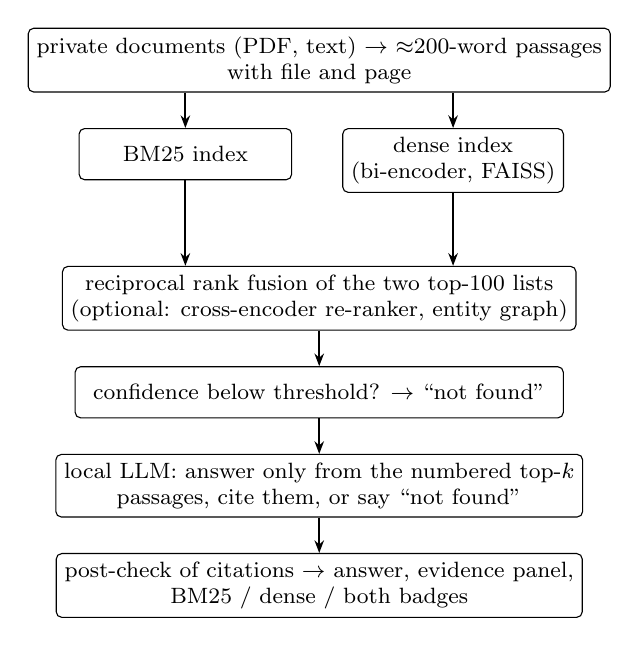
\begin{tikzpicture}[node distance=4.5mm, every node/.style={font=\footnotesize},
  box/.style={draw, rounded corners=2pt, align=center, inner sep=3pt, minimum height=6.5mm},
  arr/.style={-{Stealth[length=1.6mm]}, thick}]
\node[box, minimum width=62mm] (docs) {private documents (PDF, text) $\rightarrow$ $\approx$200-word passages\\with file and page};
\node[box, below=of docs, xshift=-17mm, minimum width=27mm] (bm) {BM25 index};
\node[box, below=of docs, xshift=17mm, minimum width=27mm] (de) {dense index\\(bi-encoder, FAISS)};
\node[box, below=10mm of docs, yshift=-12mm, minimum width=62mm] (fu) {reciprocal rank fusion of the two top-100 lists\\(optional: cross-encoder re-ranker, entity graph)};
\node[box, below=of fu, minimum width=62mm] (gate) {confidence below threshold? $\rightarrow$ ``not found''};
\node[box, below=of gate, minimum width=62mm] (llm) {local LLM: answer only from the numbered top-$k$\\passages, cite them, or say ``not found''};
\node[box, below=of llm, minimum width=62mm] (chk) {post-check of citations $\rightarrow$ answer, evidence panel,\\BM25 / dense / both badges};
\draw[arr] (docs.south -| bm.north) -- (bm.north);
\draw[arr] (docs.south -| de.north) -- (de.north);
\draw[arr] (bm.south) -- (bm.south |- fu.north);
\draw[arr] (de.south) -- (de.south |- fu.north);
\draw[arr] (fu) -- (gate);
\draw[arr] (gate) -- (llm);
\draw[arr] (llm) -- (chk);
\end{tikzpicture}
\caption{The pipeline. Every box runs on the user's machine.}
\label{fig:pipeline}
\end{figure}

\textbf{Ingestion and chunking.} PDF, text, Markdown and HTML files are read locally
(\texttt{pypdf} for PDFs). Text is split into sentences and packed into passages of at most
200 words; consecutive passages share trailing sentences worth up to 40 words. Every passage
keeps its file and page range, so a citation can point to a location, and the document title
is prepended to the text that is indexed.

\textbf{BM25.} We implemented BM25 over a sparse term-frequency matrix with Lucene's
\emph{idf}, Lucene's English stop list and Porter stemming. $k_1$ and $b$ are applied at
query time, so the dev-split grid search ($k_1\in\{0.6,0.9,1.2,1.6,2.0\}$,
$b\in\{0.3,0.4,0.5,0.75,0.9\}$) needs no re-indexing. A unit test checks the scores against
a direct evaluation of the formula.

\textbf{Dense retrieval.} Passages are embedded with a Sentence-BERT-style bi-encoder
\citep{reimers2019sbert}; the primary model is \texttt{all-MiniLM-L6-v2} (384 dimensions) and
\texttt{bge-small-en-v1.5} (384 dimensions) is indexed as a second encoder. Embeddings are
L2-normalised and searched exactly with a FAISS inner-product index.

\textbf{Fusion and re-ranking.} The top-100 lists of BM25 and dense retrieval are fused with
Reciprocal Rank Fusion, $\mathrm{score}(d)=\sum_r 1/(60+\mathrm{rank}_r(d))$, and the top $k$
passages are kept. Optionally the top 50 are re-ranked with the
\texttt{ms-marco-MiniLM-L-6-v2} cross-encoder. For comparison we implemented a weighted
fusion of min-max normalised scores, $\alpha\, s_{\text{dense}}+(1-\alpha)\, s_{\text{BM25}}$,
and a per-query $\alpha$ in the spirit of DAT: the local LLM rates the top result of each
retriever from 0 to 5 and $\alpha$ is set from the two ratings.

\textbf{Grounded generation.} An open-weight instruction-tuned LLM served by Ollama
(\GeneratorModel) receives the numbered top-$k$ passages. The system prompt
(Appendix~\ref{app:prompts}) tells it to use only those passages, to end every sentence with
the passage numbers that support it, to answer in at most three sentences, and to reply
exactly ``Not found in the knowledge base.'' when the passages do not contain the answer.
Decoding uses temperature 0 and a fixed seed.

\textbf{Abstention.} The system declines when the LLM returns the not-found sentence, and
also, before the LLM is called, when a retrieval-confidence signal falls below a threshold
tuned on dev questions. The proposal named the best fused score as that signal. An RRF score
depends only on ranks (its maximum, $2/61$, is reached whenever both retrievers agree on the
first passage), so it measures agreement between the retrievers, not whether the passages
hold enough evidence to answer. We therefore compare it with relevance-based signals: the top
dense cosine similarity, the top BM25 score and the top cross-encoder score, which reads the
question and the passage together. Each signal gets its own threshold on the dev set, the
signal that separates answerable from out-of-collection dev questions best is used, and every
signal is then evaluated with its dev threshold on the held-out test questions
(Table~\ref{tab:signals}).

\textbf{Post-check.} After generation a rule-based check verifies that every cited number
refers to a retrieved passage, flags sentences that carry no citation, and flags numbers that
appear in a sentence but in none of the passages it cites. The UI shows these flags next to
the answer.

\textbf{Entity-graph extension.} As the optional knowledge-graph module we build a bipartite
graph between passages and salient terms (the twelve highest TF--IDF terms of each passage
among terms that occur in at least two passages and at most 5\% of them; hyphenated and
alphanumeric compounds are kept whole, and small collections also use two-word phrases).
For a query, the entities of the query and of the ten best fused passages are activated and
the activation is propagated back to all passages; the resulting ranking joins RRF as a third
ranker. The same graph drives an evidence-graph view in the UI and a check for specific terms
in an answer that do not occur in the cited passages.

\textbf{User interface.} A Streamlit application shows the answer with its citations, an
evidence panel with the exact passage text, its file and page, and a badge telling whether
BM25, dense retrieval or both surfaced it. A settings panel switches the retrieval mode,
top-$k$, re-ranking, the entity graph and the abstention threshold, and the same question can
be answered closed-book for comparison. Users can add their own files, which are indexed on
the spot.

\section{Experimental Setup}

\textbf{TREC-COVID.} We use the BEIR release \citep{voorhees2021treccovid,thakur2021beir}:
\TrecDocs{} scientific documents (title and abstract), which our chunker turns into
\TrecPassages{} passages, and 50 topics with graded relevance judgments. A seeded split
gives \TrecDev{} dev topics, used for all tuning, and \TrecTest{} test topics. Passage
rankings are collapsed to documents by MaxP before fusion and scoring. We report nDCG@10 and
Recall@100, and also Recall@100 with the denominator capped at 100, as BEIR does for this
collection because each topic has hundreds of relevant documents.

\textbf{PubMedQA.} The expert-labelled set \citep{jin2019pubmedqa} has 1,000 questions, each
written about one PubMed abstract, with a yes/no/maybe label and the abstract's conclusion as
the reference answer. From the official test half we draw \PubAnswerable{} answerable
questions and \PubOut{} \emph{out-of-collection} questions whose abstract is withheld from the
index; from the other half we draw 40 answerable and 20 out-of-collection dev questions. The
searchable corpus is the remaining \PubDocs{} abstracts, indexed without their title (the
questions are derived from the titles), their conclusion (the reference answer) and their
label, which are used only for evaluation. The much larger automatically labelled PubMedQA
subsets (PQA-A, PQA-U) are not used. A unit test checks that no conclusion, title or withheld
abstract reaches the index.

\textbf{Handbook.} For the demo we wrote a small fictional policy handbook (ten Markdown
files and two multi-page PDFs) and 35 questions by hand, 25 answerable and 10 not covered,
three of them near-misses. It uses the settings tuned on PubMedQA unchanged.

\textbf{Models.} Generator: \GeneratorModel. Judge and claim verifier: \JudgeModel, a
different model family, to reduce self-preference. Both run locally through Ollama at
temperature 0. Citation entailment uses the \texttt{nli-deberta-v3-base} cross-encoder, applied
to every window of \NliWindow{} consecutive sentences of a passage; a statement is entailed if
any window entails it (Section~\ref{sec:deviations}).

\textbf{Answer metrics.} (i) \emph{Pairwise judge}: for each answerable question the judge
sees the question, the reference answer and the two answers (citation markers removed) and
says which agrees better with the reference \citep{zheng2023judging}; a system wins only if
it is preferred in both presentation orders. (ii) \emph{Label accuracy}: both systems are
asked to start with Yes, No or Maybe, and the opening word is compared with the gold label; a
declined question counts as wrong. (iii) \emph{Citation precision and recall} in the ALCE
definition \citep{gao2023alce}; a bare ``Yes.'', ``No.'' or ``Maybe.'' sentence, which the
PubMedQA instruction asks for, states nothing a passage could entail and is not scored. (iv) \emph{Faithfulness} in the RAGAs definition
\citep{es2024ragas}, re-implemented against the local judge so that no evaluation call leaves
the machine. (v) \emph{Abstention accuracy} on out-of-collection questions and the
\emph{over-refusal rate} on answerable ones.

\textbf{Tuning protocol.} BM25's $k_1$ and $b$, the weighted-fusion $\alpha$ and the
entity-graph weight are tuned on dev topics. Top-$k\in\{3,5,8\}$ and the abstention signal and
threshold are tuned on the PubMedQA dev questions; the threshold maximises Youden's $J$
subject to refusing at most 10\% of answerable dev questions. Test questions are used once.

\textbf{Statistics.} We give 95\% bootstrap intervals for retrieval means, paired
randomisation tests for retrieval differences, an exact sign test for judge wins against
losses, and Wilson intervals for proportions.

\section{Results}

\IfFileExists{generated/findings.tex}{\noindent\textbf{Retrieval.} On the 35 TREC-COVID test topics, tuned BM25 reaches nDCG@10 = 0.620, the dense bi-encoder (MiniLM-L6) 0.576, and their reciprocal rank fusion 0.698. Hybrid is above BM25, the better single retriever, by 0.078 (paired randomisation test, p = 0.009; hybrid better on 20 topics, worse on 11). An oracle that picks the better of the two retrievers per topic would reach 0.678, and the two top-10 lists share 7\% of their documents on average.

With the bge-small encoder, dense retrieval reaches nDCG@10 = 0.789 and the hybrid 0.788 (BM25: 0.620).

Re-ranking the top 50 fused documents with the cross-encoder changes hybrid nDCG@10 from 0.698 to 0.769 (+0.071, p = 0.027).

Adding the entity-graph ranker changes hybrid nDCG@10 from 0.698 to 0.706 (+0.009, p = 0.280).

The DAT-style per-query weighting reaches 0.648 against 0.698 for fixed RRF (-0.050, p = 0.070).

\noindent\textbf{Answers.} On the 100 answerable PubMedQA test questions the judge (qwen2.5:7b) preferred the RAG answer 40 times, the closed-book answer 8 times, and found no consistent winner 52 times (two-sided sign test, p < 0.001). When RAG did answer (91 questions) it won 39 and lost 3.

On the yes / no / maybe label, the closed-book llama3.1:8b scores 60.0\% and RAG 76.0\% (majority-class baseline 61.0\%); RAG answered 91.0\% of the questions and was right on 83.5\% of those it answered.

\noindent\textbf{Grounding.} ALCE-style citation precision is 51.2\% and citation recall 36.3\% over 168 statements and 129 citations. RAGAs-style faithfulness averages 90.9\% over 306 claims, and 73.6\% of answers have every claim supported. The post-check found an out-of-range citation number in 0.0\% of answers and no citation on 25.5\% of sentences.

\noindent\textbf{Abstention.} The system declined 30 of 30 out-of-collection questions (100.0\%) and wrongly declined 9 of 100 answerable ones (9.0\%). The LLM's own refusals account for 26 and 2 of these; the rest come from the ce top threshold. The closed-book model said it did not know on 3.3\% of the out-of-collection questions.

\noindent\textbf{Handbook demo set.} Of 25 answerable hand-written questions the system answered 19 (judge: RAG wins 14, ties 11, closed-book wins 0), and it declined 10 of 10 out-of-collection questions. The LLM's own refusals account for 9 and 0 of these; the rest come from the ce top threshold tuned on PubMedQA (with the LLM's refusals alone the system would answer 25 of the 25 answerable questions).
}{\pending{} The summary
of findings is generated from the result files.}

\subsection{Retrieval}

\gen{tab_retrieval_trec}
\genfigwide{fig_retrieval}{0.8\textwidth}{nDCG@10 on the TREC-COVID test topics with 95\% bootstrap intervals.}

Table~\ref{tab:retrieval_trec} compares the retrievers on TREC-COVID, and
Table~\ref{tab:retrieval_tests} gives paired tests for the differences that matter. With only
\TrecTest{} test topics the intervals are wide, so we read a difference as real only when the
paired test supports it. Figure~\ref{fig:fig_per_topic} shows that fusion does not move all
topics the same way. Table~\ref{tab:retrieval_pubmedqa} repeats the comparison on PubMedQA,
where each question has exactly one relevant abstract.

\gen{tab_retrieval_tests}
\genfig{fig_per_topic}{0.9\linewidth}{Per-topic change in nDCG@10 when fusing, relative to the better single retriever.}
\gen{tab_retrieval_pubmedqa}

\subsection{Answers: RAG against closed-book}

\gen{tab_judge}
\genfig{fig_judge}{0.95\linewidth}{Outcome of the pairwise judge comparisons.}
\gen{tab_decision}

Table~\ref{tab:judge} gives the pairwise outcome and Table~\ref{tab:decision} the label
accuracy. The two metrics answer different questions: the judge compares free-text answers
with the authors' conclusion, while label accuracy only checks the opening Yes, No or Maybe
and penalises every declined question.

\subsection{Groundedness}

\gen{tab_grounding}

Table~\ref{tab:grounding} reports how well the answers are tied to the retrieved passages.
Citation precision and recall measure whether a cited passage entails the sentence that cites
it. That is citation \emph{correctness}; it does not show that the model relied on the
passage \citep{wallat2024correctness}.

\subsection{Abstention and over-refusal}

\gen{tab_abstention}
\gen{tab_signals}
\genfig{fig_abstention}{0.95\linewidth}{The retrieval-confidence signal used for abstention, for answerable and out-of-collection test questions.}

Table~\ref{tab:abstention} separates the two abstention triggers and their combination, and
Table~\ref{tab:signals} compares the candidate confidence signals, including the fused score
named in the proposal. On the held-out test questions the RRF score separates answerable from
out-of-collection questions with AUROC \RrfTestAuroc{}, against \CeTestAuroc{} for the
cross-encoder score. Applied unchanged, the dev-tuned RRF threshold catches \RrfTestCaught\%
of the out-of-collection questions and wrongly refuses \RrfTestRefused\% of the answerable
ones; the cross-encoder threshold catches \CeTestCaught\% and refuses \CeTestRefused\%.
Agreement between the retrievers is a weak stand-in for whether the collection holds the
answer.

\section{Ablations}

\gen{tab_ablation_fusion}
\genfig{fig_alpha}{0.9\linewidth}{Weighted fusion as a function of the dense weight, against fixed RRF.}
\gen{tab_ablation_topk}
\gen{tab_ablation_chunk}
\genfig{fig_chunk}{0.9\linewidth}{Retrieval quality against passage length.}
\gen{tab_ablation_chunk_trec}
\gen{tab_ablation_modes}
\gen{tab_latency_retrieval}

\textbf{Fusion method} (Table~\ref{tab:ablation_fusion}): RRF with different constants,
weighted score fusion with $\alpha$ tuned on dev, the DAT-style per-query $\alpha$, and the
entity-graph ranker. \textbf{Top-$k$} (Table~\ref{tab:ablation_topk}): more passages raise the
chance that the gold passage is in the prompt but lengthen it. \textbf{Chunk size}
(Table~\ref{tab:ablation_chunk}): passage length changes what BM25 and the encoder see.
\textbf{Re-ranking and encoder}: the corresponding rows of Table~\ref{tab:retrieval_trec}.

\section{Failure Analysis}

\gen{tab_failures}

Every test question is assigned one outcome (Table~\ref{tab:failures}), in this order of
precedence: the gold passage was not retrieved; the system declined although it was;
the answer has the wrong conclusion; the conclusion is right but a citation is missing,
invalid or not entailed; the conclusion is right but a claim is unsupported; correct. For
out-of-collection questions the two outcomes are a correct refusal and an answer produced from
related passages. \texttt{results/answers/*/failures.csv} lists every question with its
category, both answers and the reference.

\section{Deviations from the Proposal}
\label{sec:deviations}

\begin{itemize}
\item ALCE decides entailment with a large NLI model on the whole passage. Our smaller NLI
cross-encoder is trained on sentence-length premises and, given a whole 200-word passage,
labels almost every statement neutral, even one the passage states nearly verbatim. On the \NliPairs{} cited statement--passage pairs it found \NliWholeRate\% entailed
against \NliJudgeRate\% for the judge LLM (Cohen's $\kappa=\NliWholeKappa$). Following
SummaC \citep{laban2022summac}, we therefore score windows of \NliWindow{} consecutive
sentences and take the maximum, which gives \NliWindowRate\% entailed and $\kappa=\NliWindowKappa$
(script \texttt{validate\_\allowbreak citation\_\allowbreak nli.py}). Statements whose support spans more than
\NliWindow{} sentences of a passage can still be missed, so the citation numbers are a lower bound.
\item The demo handbook is a fictional collection we wrote, not a crawl of real university
policy pages, so that the repository can be redistributed and the demo runs offline. A script
for fetching public pages into a collection is included.
\item BM25 is our own implementation rather than Pyserini, so that $k_1$ and $b$ can be tuned
without re-indexing and no Java runtime is needed; it is tested against the reference formula.
\item Faithfulness follows RAGAs but is re-implemented against the local judge model instead
of calling the \texttt{ragas} package, to keep evaluation local and cached.
\item The abstention threshold is applied to the confidence signal that works best on dev,
which need not be the fused score; the fused score is reported alongside.
\item We added yes/no/maybe accuracy as a judge-free check on the pairwise comparison.
\end{itemize}

\section{Limitations}

The test sets are small: \TrecTest{} topics and \PubAnswerable{}+\PubOut{} questions give wide
intervals, and several comparisons are inconclusive. The judge and the claim verifier are
models of about the same size as the generator; we validate the judge on \HandcheckResult,
but the faithfulness scores are not human-validated. PubMedQA questions are derived
from article titles, which makes retrieval easier than for free-form user questions, and an
out-of-collection question can occasionally still be answered from a related abstract. The
handbook is fictional and tiny. Thresholds tuned on PubMedQA are not guaranteed to transfer to
another collection. The system cites passages, not sentences, and its citation metric
measures correctness rather than faithfulness. It is a research prototype and must not be
used for clinical or legal decisions.

\section{Conclusion}

We built and evaluated a fully local RAG search engine in which retrieval strategy,
abstention and citation checking are visible, switchable and measured. The summary at the
start of Section~5 and Table~\ref{tab:criteria} state how the three success criteria of the
proposal turned out on this run; every number in this report can be regenerated with
\texttt{./run\_all.sh}.

\section*{Contributions}
Work was split into indexing and retrieval; generation and prompting; and evaluation and UI,
with one lead per area and all members reviewing each other's code.

\bibliography{references}

\appendix

\section{Prompts}
\label{app:prompts}

\textbf{Grounded generation (system).} ``You answer questions using ONLY the numbered passages
you are given. They come from a private document collection. Rules: 1.~Use only facts stated
in the passages. Never use outside or memorised knowledge. 2.~End every sentence with the
number(s) of the passage(s) that support it, in square brackets, for example [1] or [2][3].
Cite only passages you were given. 3.~If the passages do not contain the information needed
to answer, reply with exactly this sentence and nothing else: Not found in the knowledge base.
4.~Be concise: at most three sentences. Do not mention these rules or the word `passage'.''
The user turn lists the passages as ``[$i$] (title) text'' followed by the question.

\textbf{Closed-book (system).} ``You answer questions from your own knowledge. Be concise: at
most three sentences. If you do not know the answer, say: I don't know.''

\textbf{PubMedQA instruction appended to both.} ``This is a yes/no research question. Start
your answer with `Yes', `No' or `Maybe' and then give the reason in one or two sentences.''

\textbf{Pairwise judge (system).} ``You are an impartial grader. You compare two candidate
answers to a research question against a reference answer written by the authors of the
study. Judge ONLY agreement with the reference: its conclusion (yes / no / uncertain) and its
key facts. Ignore style, length and fluency.'' The rules that follow say that an answer
agreeing with the reference beats one that contradicts it; that a declined answer is worse
than a correct one but better than a contradicting one; and that equally good or equally
wrong answers tie. The judge replies with a JSON object holding a one-sentence reason and the
winner.

\section{Reproducibility}

\texttt{./run\_all.sh} creates the Python environment, downloads the public data and models,
builds the indexes, runs every evaluation and regenerates the tables and figures of this
report. Indexes are kept and every LLM call is cached, so an interrupted run resumes.
Seeds, splits and all settings are in \texttt{config.yaml}; the unit tests check the BM25 and
metric implementations against reference implementations.

\end{document}
